% !TEX root = ../main.tex



\subsection{Positie, snelheid en versnelling}

\begin{frame}{Positie, snelheid en versnelling}
\end{frame}

\begin{frame}{Centripetale versnelling}
\begin{figure}
\href{run:./app/ECB_centripetale_versnelling.ggb}{%
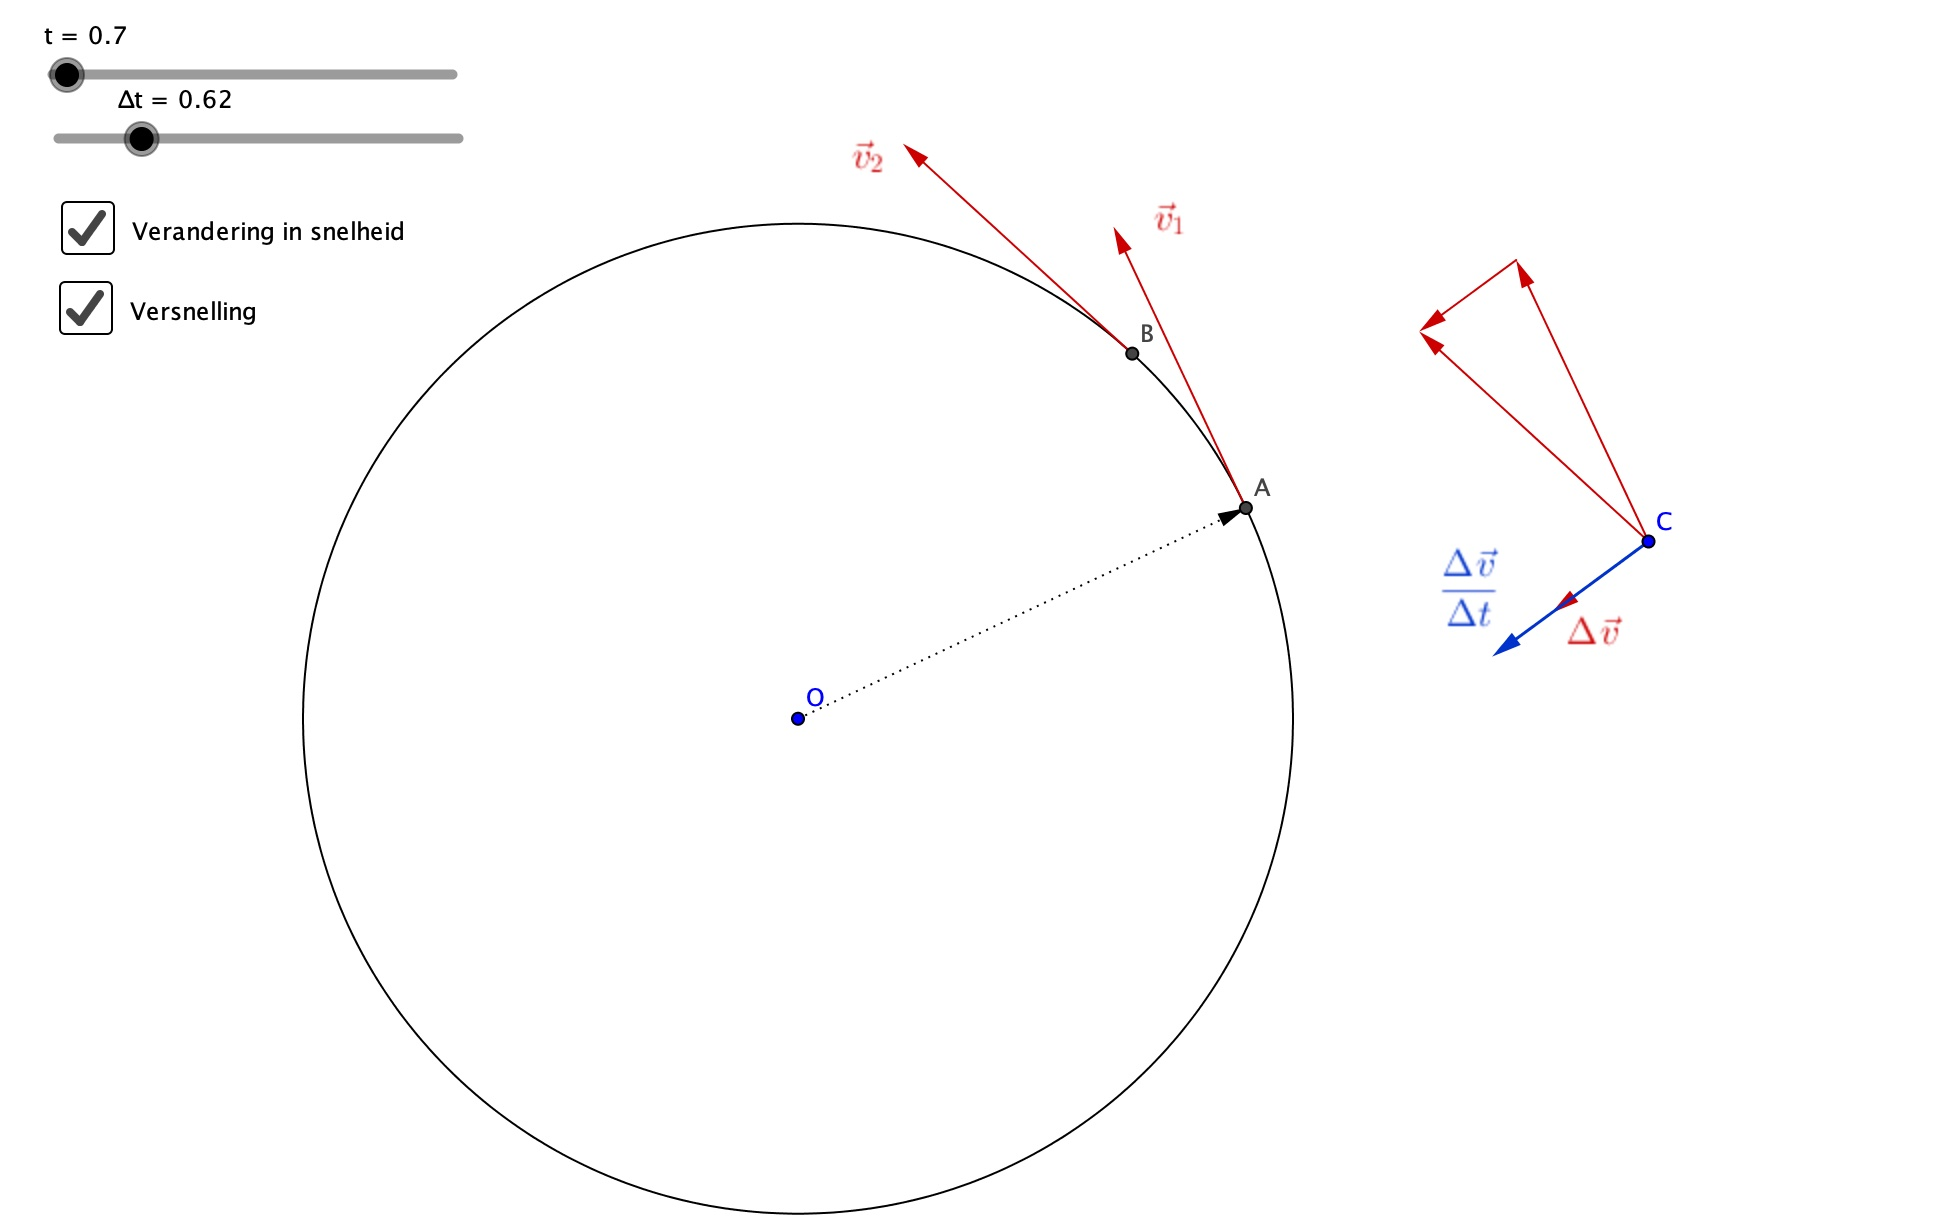
\includegraphics[height=\textheight-3\baselineskip]{ECB_centripetale_versnelling}%
}
\end{figure}
\end{frame}


\subsection{Oefeningen}

\usebackgroundtemplate{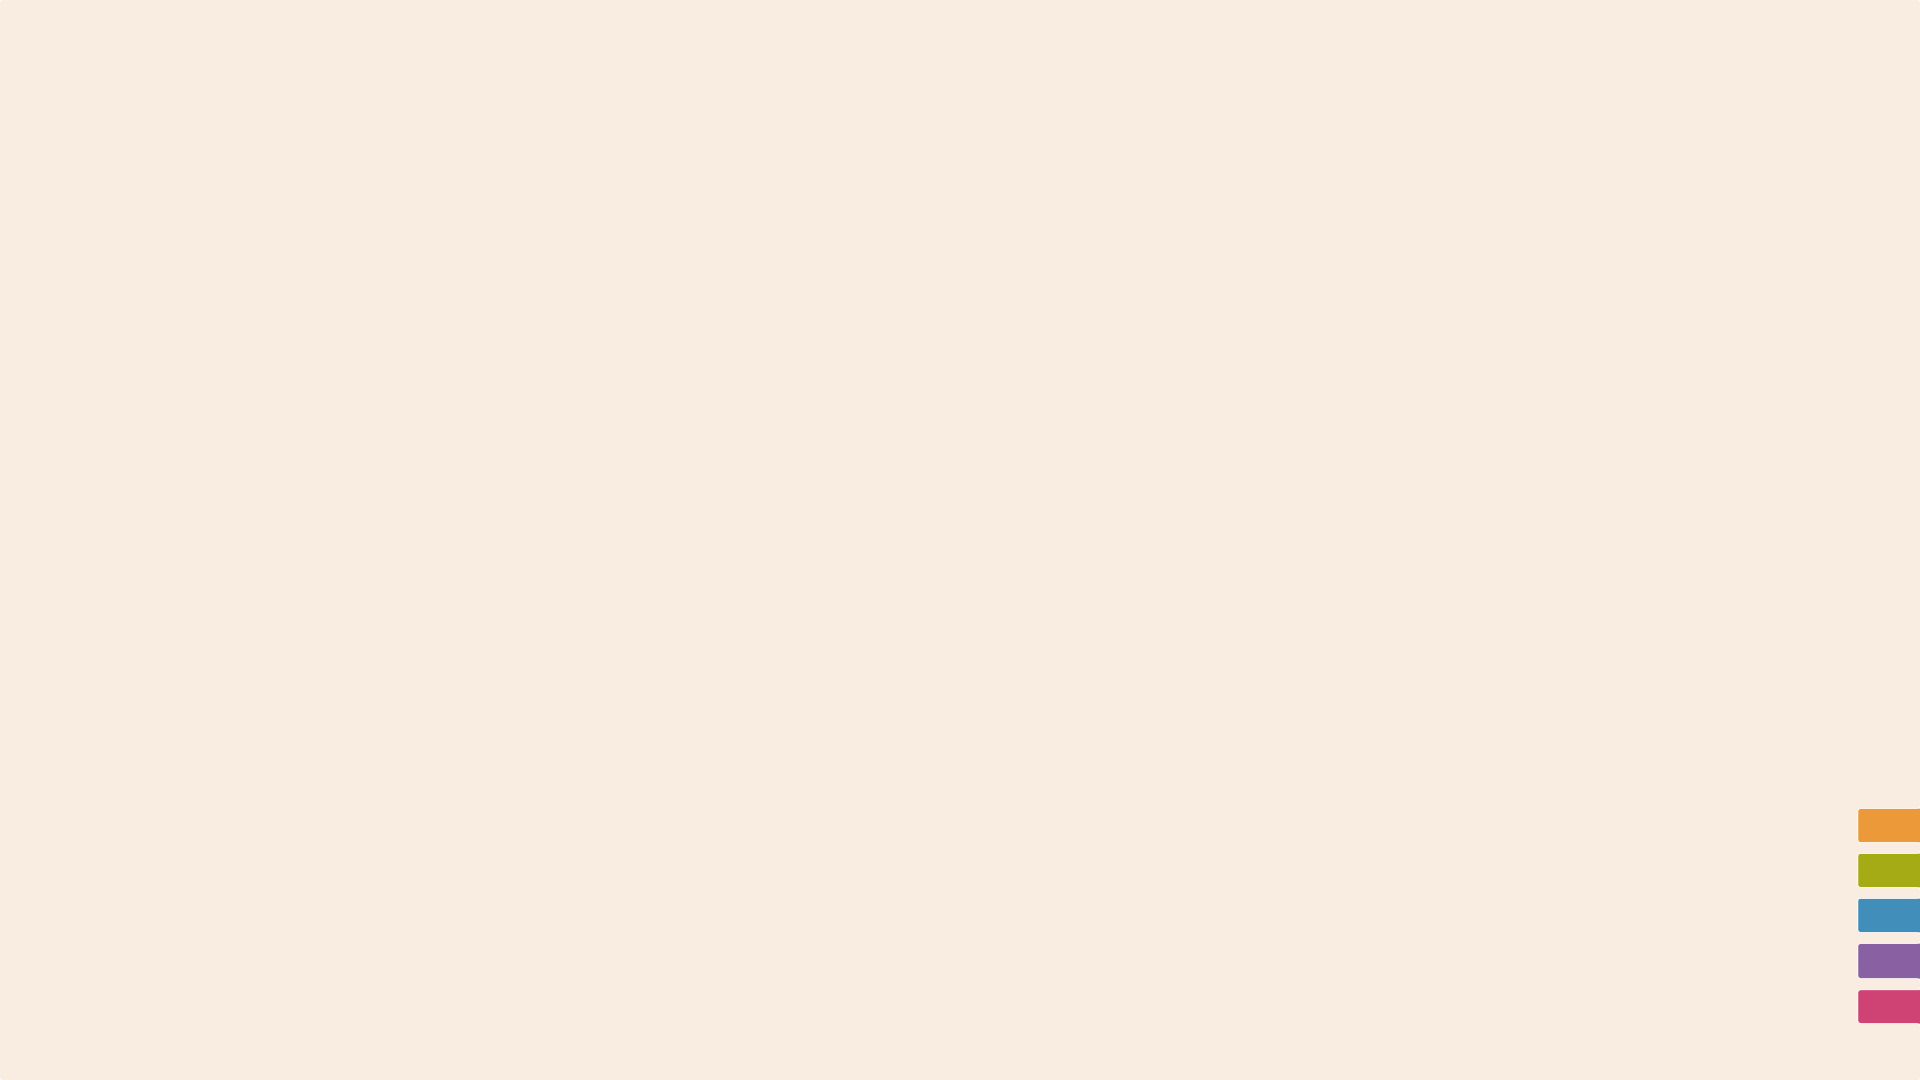
\includegraphics[width=\paperwidth,height=\paperheight]{achtergrond22n_FV}}

\begin{frame}{Voorbeeldoefening}
Een auto rijdt door een bocht met een snelheid van \SI{50}{km/h}. Heef de auto een andere versnelling wanneer hij diezelfde bocht neemt met een snelheid van \SI{70}{km/h}?% Licht je antwoord toe.
\begin{enumerate}
\item Ja
\item Nee
\end{enumerate}

\end{frame}

\begin{frame}{Voorbeeldoefening}
Als een auto met \SI{60}{km/h} een scherpe bocht neemt, en daarna met dezelfde snelheid een flauwe bocht, is de versnelling dan in beide gevallen gelijk?% Leg uit.
\begin{enumerate}
\item Ja
\item Nee
\end{enumerate}
\end{frame}



\begin{frame}{Oefening 8 p. 95}
\begin{columns}[T]
    \begin{column}{0.5\textwidth}
    	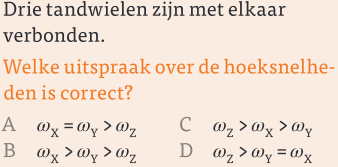
\includegraphics[width=\textwidth]{8p95_1}
    \end{column}
    \begin{column}{0.5\textwidth}
    	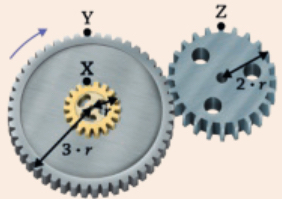
\includegraphics[width=\textwidth]{8p95_2}
    \end{column}
\end{columns}
\end{frame}


\begin{frame}{Oefening 8 p. 93}
\begin{figure}
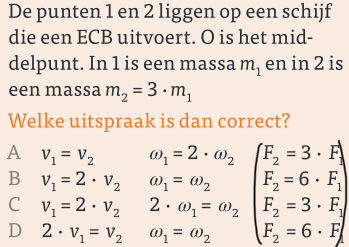
\includegraphics[width=0.6\textwidth]{8p93_1}%
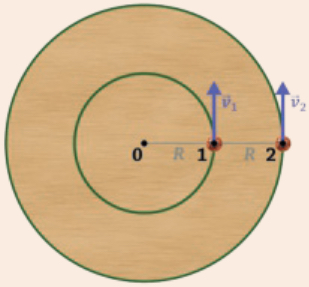
\includegraphics[width=0.4\textwidth]{8p93_2}
\end{figure}
\end{frame}


\begin{frame}{Oefening 9 p. 95}
\begin{columns}[T]
    \begin{column}{0.5\textwidth}
    	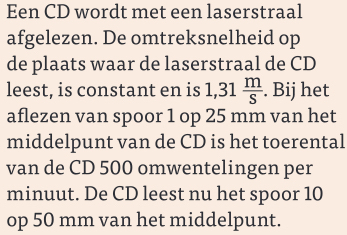
\includegraphics[width=\textwidth]{9p95_1}
    \end{column}
    \begin{column}{0.5\textwidth}
    	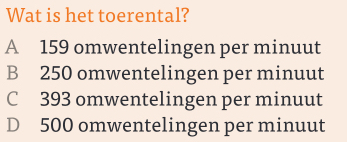
\includegraphics[width=\textwidth]{9p95_2}
    \end{column}
\end{columns}
\end{frame}

\note{Antwoord B is correct. $\omega_2=\frac{r_1}{r_2}\omega_1=\frac{1}{2}\omega_1$}

\begin{frame}{Voorbeeldoefening}
Bereken de hoeksnelheid van de aarde om haar as. Bereken de snelheid van een punt van het aardoppervlak:
\begin{enumerate}
\item aan de evenaar,
\item op \SI{51}{\degree} noorderbreedte.
\end{enumerate}
\end{frame}

\begin{frame}{Voorbeeldoefening}
\begin{columns}[T]
    \begin{column}{0.5\textwidth}
    	Bereken de hoeksnelheid van de aarde om haar as. Bereken de snelheid van een punt van het aardoppervlak:
		\begin{enumerate}
			\item aan de evenaar,
			\item op \SI{51}{\degree} noorderbreedte.
		\end{enumerate}
    \end{column}
    \begin{column}{0.5\textwidth}
    	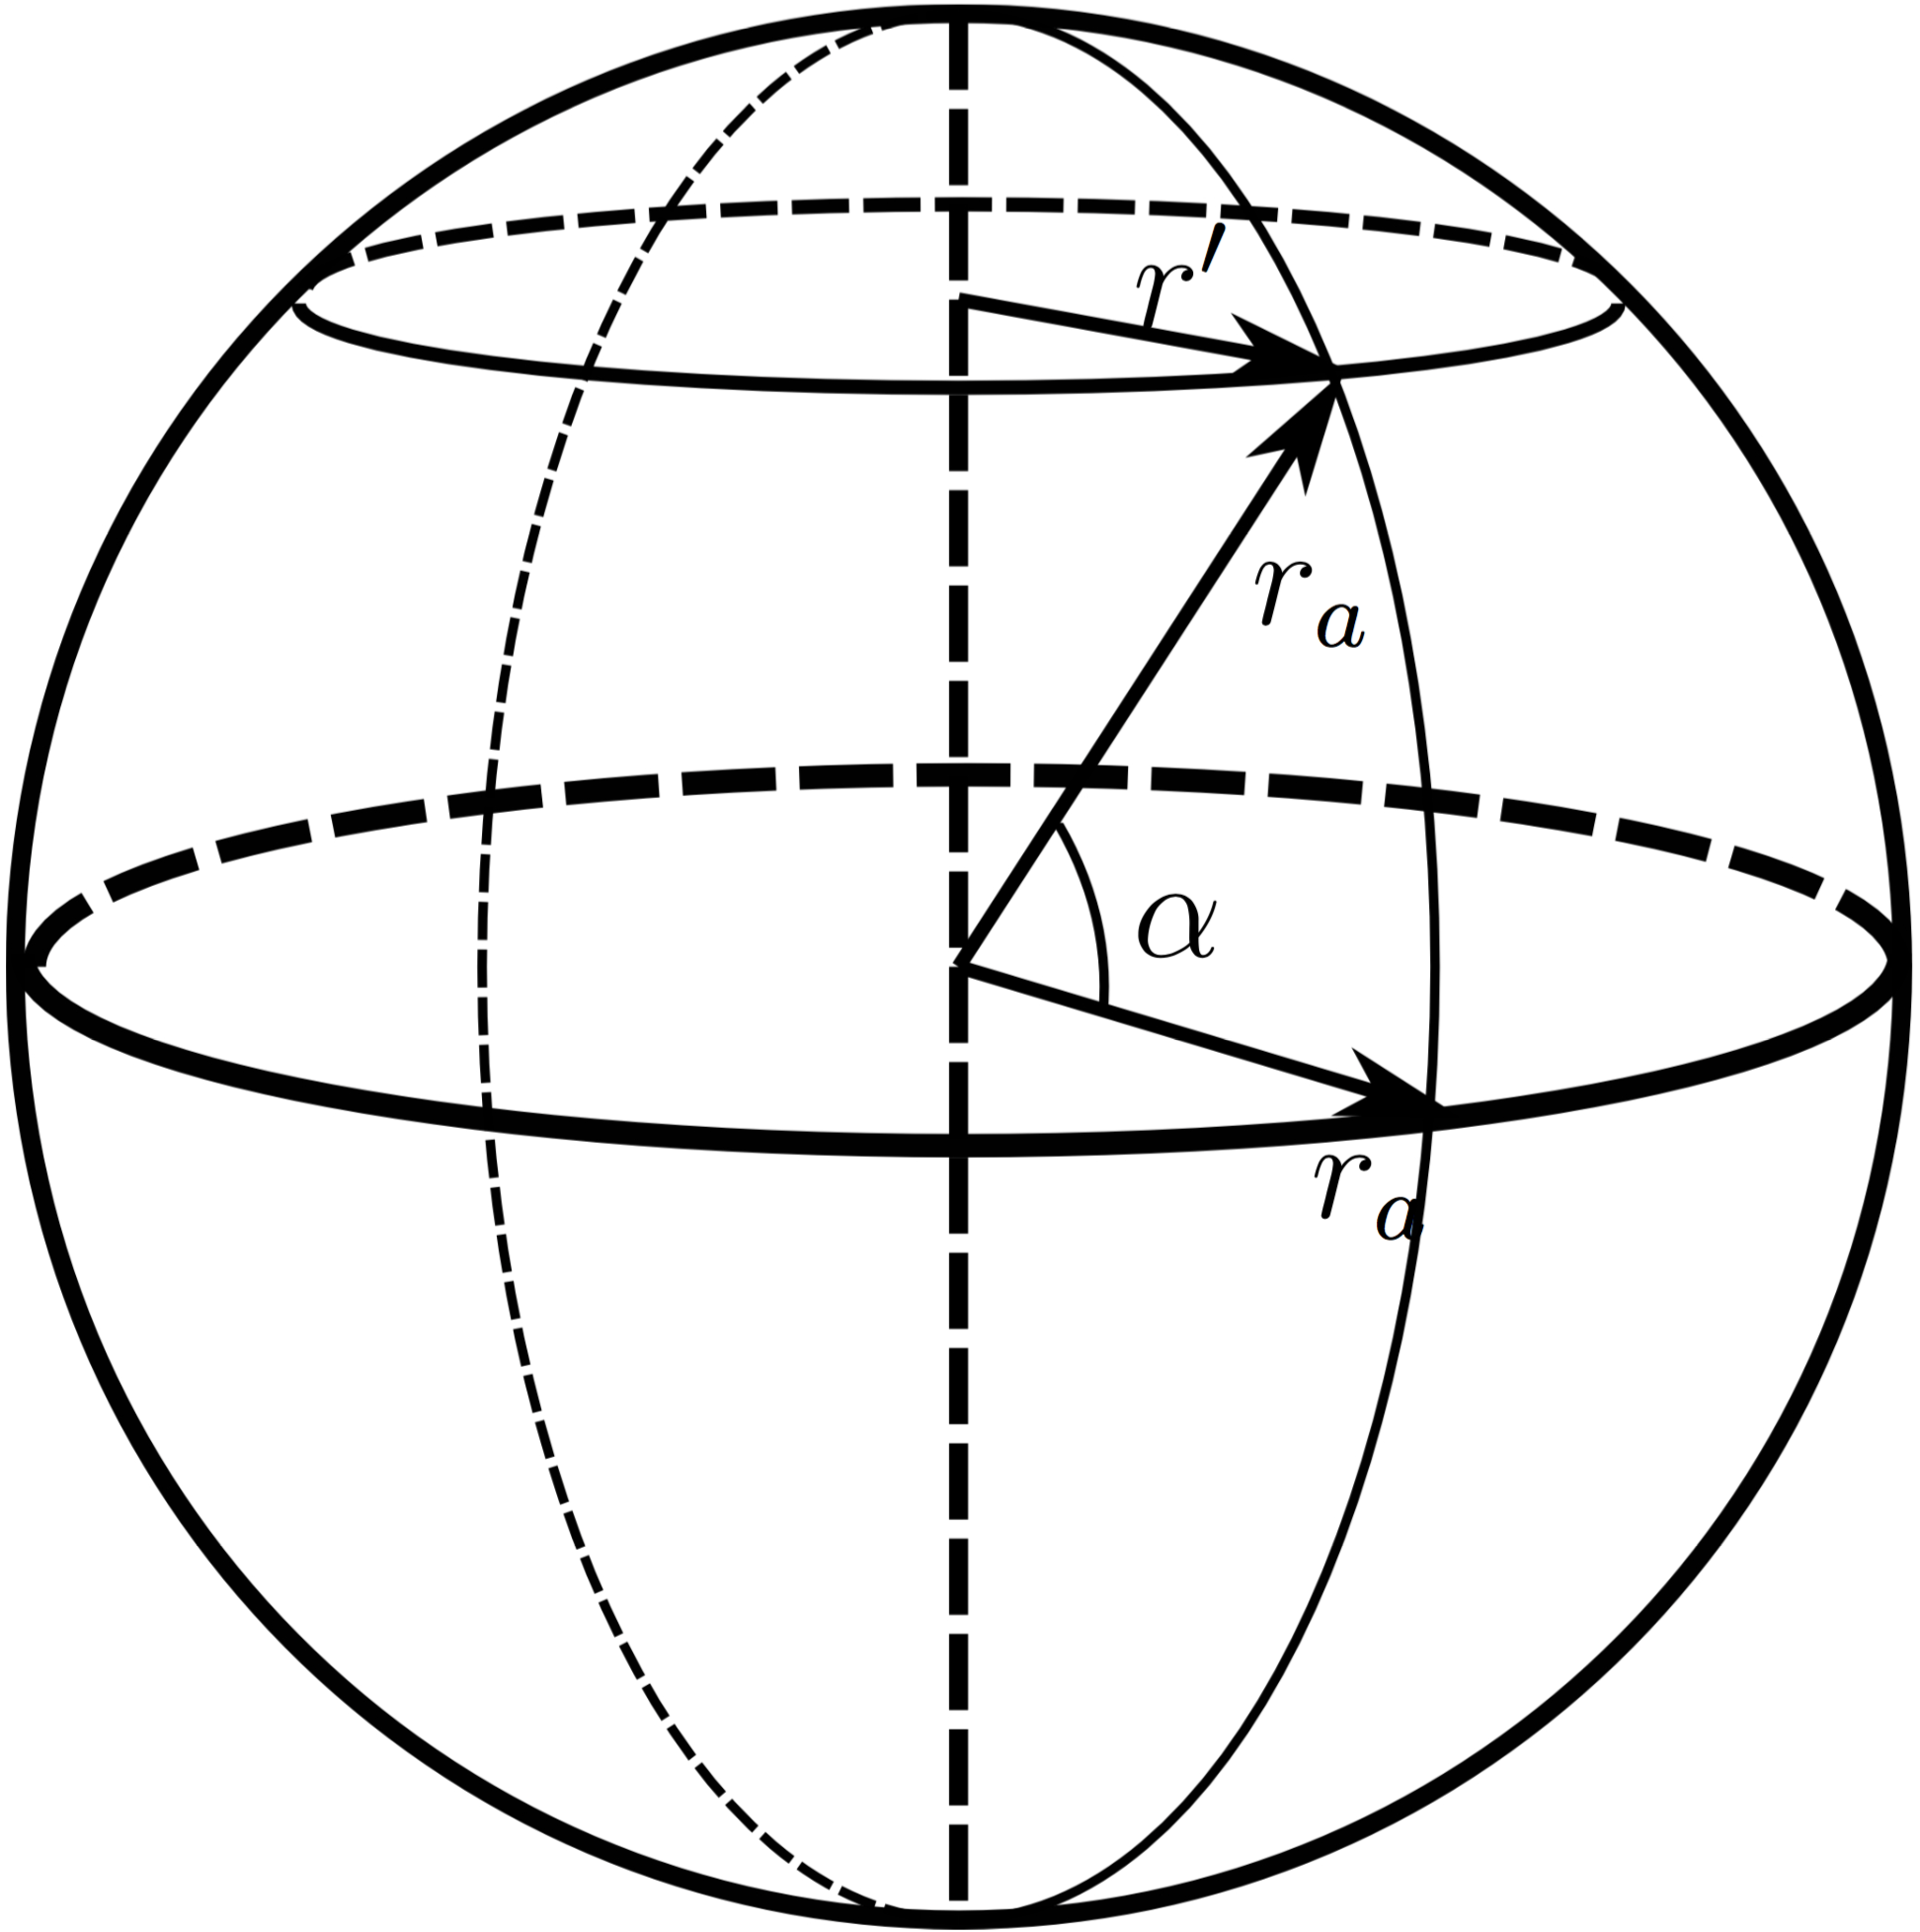
\includegraphics[width=\textwidth]{aardehoeksnelheid2.png}
    \end{column}
\end{columns}
\end{frame}


\usebackgroundtemplate{
\includegraphics[width=\paperwidth,height=\paperheight]{achtergrond22n}}
